\subsection*{Indicadores financieros}
\addcontentsline{toc}{subsection}{Indicadores financieros}

Los indicadores financieros se basan en la comparación de dos valores esenciales dentro de los documentos internos de la empresa: el \textit{balance general} y el \textit{presupuesto de la empresa}. Gracias a los indicadores financieros y a su correcta interpretación, una empresa puede identificar el rumbo que debe tomar con base en los datos históricos analizados.

Dentro de los indicadores financieros considerados, se encuentran los siguientes:

\begin{itemize}
	\item \textbf{Razón corriente:} Permite determinar la capacidad que tiene la compañía para cubrir sus deudas con los activos disponibles.
	
	\item \textbf{Nivel de endeudamiento total:} Determina el grado y la forma de participación que tienen los acreedores dentro de la estructura financiera de la compañía.
	
	\item \textbf{Rentabilidad operacional:} Este indicador evidencia el porcentaje de los ingresos recibidos que se convierten en beneficios después del pago de los costos operacionales.

	\item \textbf{Rentabilidad neta:} Indica el nivel de ganancias con respecto a las ventas netas una vez realizado el pago de los costos fijos y variables.
	
	\item \textbf{Rentabilidad de patrimonio:} Evidencia el nivel de ganancia que obtiene la empresa a partir de la inversión realizada por los accionistas.
\end{itemize}

En la tabla \ref{IndicadoresFinancieros} se proyectan estos indicadores a un horizonte de cinco años.

\begin{table}[H]
	\centering
	\caption[{Indicadores financieros}]{\centering Indicadores financieros. \textit{Fuente:} Autores.}
	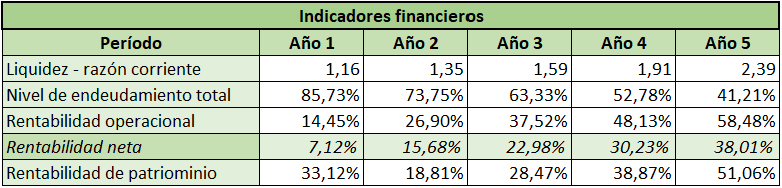
\includegraphics[width=13cm]{Imagenes/IndicadoresFinancieros.png}
	\label{IndicadoresFinancieros}
\end{table}

Adicionalmente, se analizaron los indicadores financieros VAN, TIR y la relación costo-beneficio, con el objetivo de demostrar la viabilidad de la inversión propuesta para los accionistas. Los resultados obtenidos a partir del flujo de caja deben tenerse en cuenta para interpretar los datos presentados en la tabla \ref{FlujoCajaLibre}.

\begin{table}[H]
	\centering
	\caption[{Flujo de caja libre}]{\centering Flujo de caja libre. \textit{Fuente:} Autores.}
	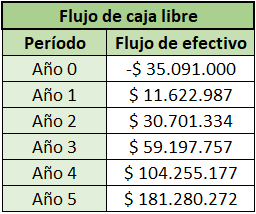
\includegraphics[width=9cm]{Imagenes/FlujoCajaLibre.png}
	\label{FlujoCajaLibre}
\end{table}

Teniendo en cuenta la tasa interna de oportunidad, entendida como la tasa mínima de rendimiento que esperan recibir los accionistas, se definió de manera estimada un valor del 15\% con el fin de compensar la inversión realizada.

\begin{table}[H]
	\centering
	\caption[{VAN, TIR y RBC}]{\centering VAN, TIR y RBC. \textit{Fuente:} Autores.}
	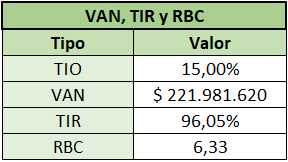
\includegraphics[width=9cm]{Imagenes/VANTIR.png}
	\label{VANTIR}
\end{table}

De acuerdo con los resultados obtenidos en el análisis financiero, el proyecto presenta viabilidad en esta área. Pero su éxito dependerá del nivel de atractivo que logre generar entre los futuros inversionistas. Esto permitirá que la empresa fortalezca su capacidad de participación en un mercado competitivo con alta demanda, lo que constituye una oportunidad significativa.

Tanto el Valor Actual Neto (VAN) como la Tasa Interna de Retorno (TIR) presentan resultados positivos a largo plazo. Asimismo, la mayor liquidez reflejada en la tabla de proyección del incremento de ventas sugiere que la compañía mejorará su capacidad financiera. A esto se suma un nivel de endeudamiento con tendencia decreciente y una rentabilidad que muestra un crecimiento sostenido a lo largo de los años.